\documentclass[]{iac}

\DeclareMathOperator{\E}{E}
\DeclareMathOperator{\prob}{p}
\DeclareMathOperator{\tr}{tr}

\newcommand{\etalia}{\textit{et al.}}
\newcommand*{\vectornorm}[1]{\left\|#1\right\|}
\newcommand*\rfrac[2]{{{}^{#1}\!/_{#2}}} % running fraction with slash - requires math mode.
\newcommand*\T{\mathsf{T}}

\begin{document}

\IACpaperyear{17}
\IACpapernumber{D9.2.8}
\IACconference{65}
\IAClocation{Toronto, Canada}
\IACcopyrightA{2014}{the authors}

\title{Technology demonstrator of a rocket carrying a deployable fleet of autonomous gliders}

%\author{Main~Author\\Affiliation, Country, email address\and
%		Co-Author\\Affiliation, Country, email address}
\IACauthor{Patrick Spieler}{Swiss Federal Institute of Technology, Lausanne, Switzerland, }
\IACauthor{Co-Author}{Affiliation, Country, email address}

\abstract{%Rewrite: Dalmir, Sorina
%NOTE: Many of the structure of paper goes to the end of introduction
%The Intercollegiate Rocket Competition (IREC) aims to gather students from across the world to design and build a rocket that reaches an altitude of 3km or 10km, carrying a 4kg of payload. As part of this competition, the Team Duster, formed by students from Swiss universities developed a rocket with a payload targeting an apogee of 3km. \\ 
%Firstly, the rocket flying to 3km will be presented, along with its design and manufacturing processes. The rocket then follows a dual-event recovery process. Firstly, the drogue (small) parachute is deployed, reducing the speed of the rocket to about 30 m/s. At the same time the separation of the nosecone occurs thereby releasing the payload. After the rocket descends to an altitude of 457 meters, the second (main) parachute is deployed, reducing the speed to 6m/s. Throughout the launch, separation, and landing phases, we constantly received telemetry (information) provided by the custom-designed avionic components placed in the nosecone of the rocket. To ensure that the deployment occurs at predefined altitudes, the decision was made to use 2 redundant systems for altitude measurement -independent of the avionics placed in the recovery bay. The trajectory of the rocket was simulated in 3 varying environments, including our own developed simulator. The rocket made its first flight towards the end of March 2017 in Switzerland where its flight data was compared with the simulation data. Based on this data, the necessary trajectory corrections were performed in order to improve the competition Flight - which occured in mid-June. \\
%Secondly, an innovative payload that flew in the rocket will also be presented. A fleet of 3 gliders are deployed from the rocket at apogee using a release based on a spring mechanism. Equipped with an autopilot, differential GPS, and control surfaces using servomotors, the gliders autonomously fly in formation. Eventually, they land at a fixed point on the ground. The gliders have. During the flight, the gliders transmit information back to the groundstation and are tracked using custom-made ground station.  Potential video-recording of the flight will be investigated in the future.
%The results of the intermediary flight (end-of-March) as well as the competition flight - both in terms of rocket trajectory and flight of the gliders - is included in the paper, along with further recommendations for a more advanced technology demonstration in the future.

The Intercollegiate Rocket Competition (IREC) aims to gather students from across the world to design and build a rocket that reaches an altitude of 3km or 10km, carrying a arbitrary payload of 4kg. As a part of this competition, team Duster, formed by students from 3 Swiss universities developed and constructed a rocket with a payload targeting an apogee of 3km. The rocket is launched by using COTS solid motor. It follows a a dual-event recovery process with first parachute deployment at apogee and second (main) parachute deployment at 457 meters.  Custom avionics inside the nosecone log and transmit information back to the ground.
Inside the rocket a payload of 4 kg is placed and that payload consists of a custom built autonomous glider ejected at apogee, which descends to a fixed point on the ground independent from the rocket. 
To estimate the apogee under variety of conditions and motor configurations 3 separate simulators are used with one being developed by the team as a part of this project. Especially interesting in this context is also the stability - both static and dynamic, which influences the design and has large impact on the performance of the rocket. 
The technology behind both the rocket and the payload together with concepts for autonomous fleet of gliders is presented and elaborated on in this paper. Design process and manufacturing, together with tests done and issues faced over the course of the project are also presented along with the solutions and recommendations for the future.
}

\maketitle
%Check for number of pages allowed, if any
\section{Introduction}

%Spaceport America Cup (formerly entitled Intercollegiate Rocket Competition (IREC)) gatheres students all over the world to participate at the biggest rocket challenge. Students are launching solid, liquid, and hybrid rockets to target altitudes of 10,000 feet (3048 meters) and 30,000 feet (9144 meters), carrying 8,8lb (3.9 kg) of payload.

%Team DUSTER, representing several Swiss universities, entered this contest to build a solid motor rocket flying to an apogee of 10,000 ft (3048 meters). The project received an honourable place 8$^th$, out of 83 teams.

%This paper contains the work developed by the team of students between November 2016 and June 2017. The first part of the article discusses the rocket design, manufacturing and flight data. The second part of the article reviews the payload placed inside the rocket. For this year, the team built a glider that was deployed at 10,000 ft and flew back to the ground. For the future, the aim is to develop a fleet of gliders that is deployed from the rocket at apogee and flies in formation back to the ground. As part of this article, the fleet of gliders will be only conceptually discussed.
Spaceport America Cup (formerly entitled Intercollegiate Rocket Competition (IREC)) gathers students from all over the world to participate at one of the biggest rocket competition. Students are launching solid, liquid, and hybrid rockets to target altitudes of 10,000 feet (3048 meters) and 30,000 feet (9144 meters), carrying 8,8lb (3.9 kg) of payload. The teams are scored according to the flight performance on the competition day, technical implementation, the quality of the report and research done as a part of the project.
Team DUSTER, representing several Swiss universities, entered this contest to build a solid motor rocket flying to an apogee of 10,000 ft (3048 meters). 
The main objective of the rocket is to achieve an apogee of 10,000 ft exactly. Deviations from this apogee result in point loss in the flight performance category. At the apogee, 2 separation events occur: separation alongside the body of the rocket where the parachutes are ejected and separation of the nosecone form the rocket. 
Recovery subsystem is responsible for obtaining this precise apogee and ensure the deployment of the parachutes. This system consists of 2 parachutes and 2 redundant instruments which are used to estimate the apogee and trigger the separation of the rocket. After the separation occurs, both parachutes are ejected from the body of the rocket and one is opened , the so-called drogue, reducing the speed of the rocket to about 30 m/s. The main parachute remains in the bag for the first part of the descend. At the same time the nosecone is also separated from the rocket and the glider is ejected. From this point the rocket consisting of 3 parts (2 body parts and the nosecone) and the glider descend independently from each other. At the altitude of 457 meters, the second (main) parachute opens, reducing the speed to 6m/s. Throughout the launch, separation and landing phases telemetry information, provided by the custom-designed avionic components placed in the nosecone of the rocket, are being constantly logged and part of them also sent to the ground station. 
In the model flown at this years competition no control mechanism were in place and also no air brakes were installed meaning once the rocket is launched the trajectory can not be influenced. This increased the importance of simulation, as the only way to determine the altitude the rocket can obtain with a chosen motor and assuming certain weather conditions.  The trajectory of the rocket was simulated in 3 varying environments, including our own developed simulator. 
The second main component of the project is the payload. The payload is an autonomous glider equipped with an autopilot, differential GPS, and control surfaces using servomotors. Its objective is to land at a fixed point on the ground and transmit data from the sensors to the ground station. In this years model only one glider had been constructed with a wing span of approximately 200mm and a body length of 100mm. The concept of multiple gliders flying in a formation is presented as well with a possibility of being implemented in next years model.  
The results of the intermediary flight (end-of-March) as well as the competition flight - both in terms of rocket trajectory and flight of the gliders - is included in the paper, along with further recommendations for a more advanced technology demonstration in the future

The structure of this paper is as follows: in the first section the rocket is presented together with 4 main subsystems: structure, avionics, propulsion and recovery. Section 2 covers the design and technology used in a glider and presents a concept of a fleet of gliders. Navigation and control, one of the main challenges in glider design, are elaborated in detail in Section XX. The last part contains the conclusion and the outlook for the future. 




\section{Rocket}


The rocket, entitled RORO I, is a 8 feet (2.45 meters) rocket propelled by a M-class solid motor. The main requirements of the rocket are presented in Table \ref{table:se_topLevelR}.

\begin{table}[h!]
\centering
\begin{tabular}{|p{0.9\columnwidth}|}
\hline
    The rocket shall achieve an apogee of 10,000 ft (3048 meters).  \\ \hline
    The rocket shall have a static margin between 1 and 2 body-calibres. \\ \hline
    The rocket shall carry a COTS barometric pressure altimeter with on-board storage as primary data source for altitude reporting.  \\ \hline
    The launch vehicle shall follow a "dual-event" recovery. \\ \hline
    The rocket shall carry a minimum mass of 8.8 lb (4 kg) of payload. \\ \hline
    The rocket shall eject its nosecone at apogee. \\ \hline
    The rocket shall release a glider from the payload section at 10 seconds after apogee. \\ \hline

\end{tabular}
\caption{Top Level Requirements for the rocket}
\label{table:se_topLevelR}
\end{table}


\subsection{Design and Manufacturing}


The rocket is divided into 3 main sub-assemblies (Figure \ref{f:rocket_adnoted}):

\begin{enumerate}[noitemsep]
    \item The nosecone - carrying avionics, the locking system for the nosecone and its ejection system
    \item The upper body - carrying the payload, the parachutes and the recovery electronics
    \item The lower body - containing logging avionics and the motor
\end{enumerate}
The rocket was designed to be robust and simple to manufacture due to the time constraints we had.
The rocket separates in the middle, between the upper and lower body to release the parachutes. Before separation the two body tubes are connected using a coupler tube.
This approach is very common in High Power Rocketry (HPR) and was chosen to minimize risk.

\begin{figure}[h!]
\centering
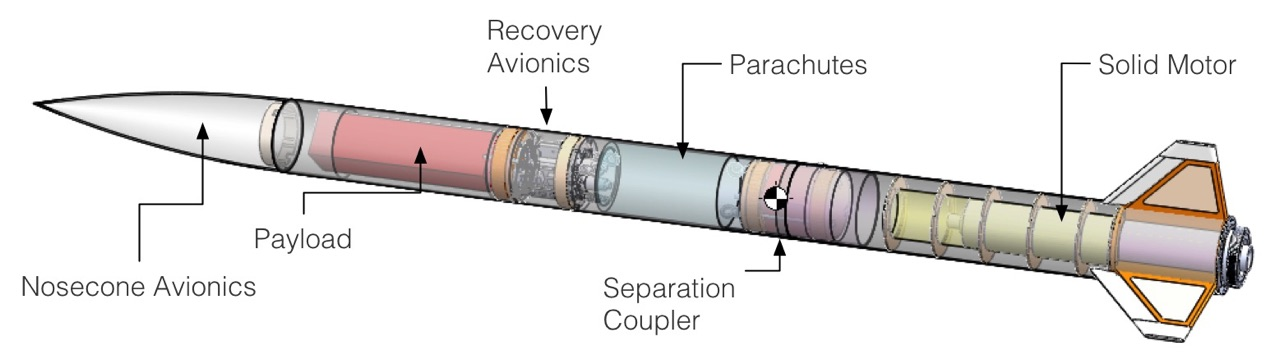
\includegraphics[width=0.5\textwidth]{img/rocket_sw_annotated.jpg}
\caption{The rocket with its main components}
\label{f:rocket_adnoted}
\end{figure}


The length as well as the diameter of the rocket were chosen to accommodate the payload which had a dimension constraint imposed by the competition and the other subsystems.

%Next, the manufacturing of each subsystem of the rocket is discussed.

% Before considering the stability in the following sections, we discuss manufacturing process of each part of the rocket.



\paragraph{Structure}
\hfill \break
The main body of the rocket is a COTS phenolic tube, reinforced with two layers of 245 g/m$^2$ twill weave carbon fibre. The reinforcement rational is determined using FEA (Finite Element Analysis), and tested during two rocket flights.
The structure contains also a coupler tube, that is made out of phenolic tube reinforced inside again with two 245 g/m$^2$ layers carbon fibre.
The rocket has two structural bulkheads, one in the lower body and one in the upper body to which the parachute cords are attached. The bulkheads are made out of two 15mm plywood plates reinforced with 4 layers of 245 g/m$^2$ carbon fibre on each side.  The bulkheads are the structurally critical elements as they transfer loads from the rocket body to the subsystems. They need to withstand both the accelerations from the launch and the parachute opening shock. 
The two bulkheads are subject to a peak load of 10kN from the parachute opening shock. An FEM analysis taking into account the  ECSS-E-HB-32-21A \cite{ecss} revealed that an additional reinforcement of the bulkheads with carbon fibre is required to sustain the loads. The analysis of the bonding to the rocket body reveals sufficient strength to sustain the opening shock.

% Dalmir, can you city the ECSS? http://www.ecss.nl/wp-content/uploads/handbooks/ecss-e-hb/ECSS-E-HB-32-21A20March2011.pdf

% Dalmir, can you city the ECSS? http://www.ecss.nl/wp-content/uploads/handbooks/ecss-e-hb/ECSS-E-HB-32-21A20March2011.pdf

% todo put the static caliber
%\paragraph{Fins}
%\hfill \break
%    The fins are sized for 1.1 calibers static stability %Reference to static/dynamic stability
 %   and were manufactured out of wood and carbon fibre, as it can be seen in Figure \ref{f:fins}. Firstly, the wood was cut at CNC (Figure \ref{f:fins} a). The inside of the fins was made out of balsa wood (Figure \ref{f:fins} b), in order to decrease the weight for higher resonance frequencies. Afterwards, on each side of each fin, 3 layers [span, chord, span] of 140 g/m$^2$ unidirectional carbon fibre were applied, to increase stiffness (Figure \ref{f:fins} c). The fins were attached to the motor tube using high temperature epoxy, reinforced with carbon fibre.

%    \begin{figure}[h!]
  %      \centering
     %   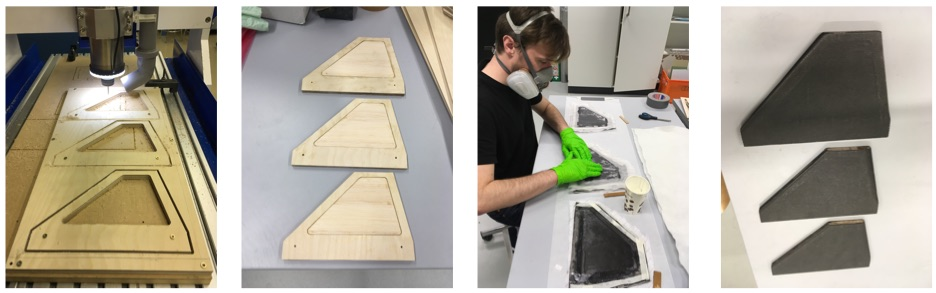
\includegraphics[width=0.5\textwidth]{img/fins.jpg}
        %\caption{a) Wood at CNC b) Final wood-made fins c) Carbon fiber manufacturing d) Final version of the fins.}
        %\label{f:fins}
    %\end{figure}
\paragraph{Fins}
\hfill \break
The fins are sized for 1.1 calibres static stability margin before liftoff.
With the burn of the motor and the corresponding mass loss the static margin increases to about 1.8 calibres.
After the first test launch and a problem with thrust alignment of the COTS motor described in section \ref{subsection:flightTests} we decided to increase the fin size in order to increase static stability.

The fins are manufactured out of wood and carbon fibre. The process is shown in Figure \ref{f:fins}. Firstly, the wood is cut at CNC (Figure \ref{f:fins} a). The inside of the fins is made out of balsa wood (Figure \ref{f:fins} b), in order to decrease the weight for higher resonance frequencies. Afterwards, on each side of each fin, 3 layers ([span, chord, span] fibre orientation) of 140 g/m$^2$ unidirectional carbon fibre are applied, to increase stiffness (Figure \ref{f:fins} c). The fins are attached to the motor tube using high temperature epoxy, reinforced with carbon fibre.
    \begin{figure}[h!]
        \centering
        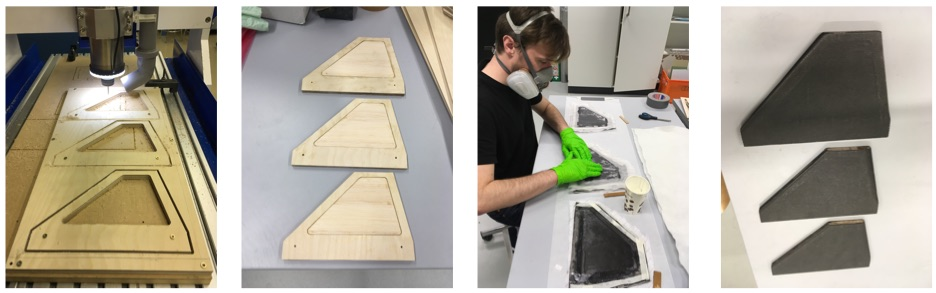
\includegraphics[width=0.5\textwidth]{img/fins.jpg}
        \caption{a) Wood at CNC b) Final wood-made fins c) Carbon fibre manufacturing d) Final version of the fins.}
        \label{f:fins}
    \end{figure}

\paragraph{Motor tube}
\hfill \break
The motor tube consists of a COTS phenolic tube. The fins are glued with 3M DP760 high-temperature epoxy to the motor tube. The tube is centred to the outer rocket body tube by six 4mm plywood centring rings distributed in equally along the motor tube.
In front of the fins, there is a 12mm CNC-cut plywood ring from which 12 M3 threaded rods connect to the thrust plate. These help holding the motor inside the rocket body during parachute opening shock.
The entire assembly can be seen in Figure \ref{f:reinforcement} c. The fins are fixed to the outer structure using ribbons of carbon fibre both on the inside and the outside of the tube, as it can be seen in Figure \ref{f:reinforcement} a,b.

  \begin{figure}[h!]
\centering
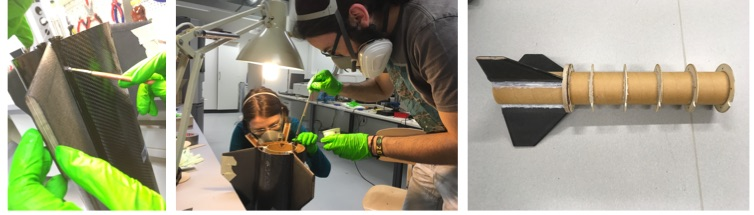
\includegraphics[width=0.5\textwidth]{img/fins_glue.jpg}
\caption{a, b) Reinforcement of the fins c)Motor tube assembly, with fins and centring rings}
\label{f:reinforcement}
\end{figure}


\paragraph{Motor case}
\hfill \break
The motor case, which is a RMS-98/7680 from Aerotech is held by a 98mm retainer from Aeropack on a custom made laser-cut aluminium thrust plate. The thrust-plate pushes directly on the fins which go through the body tube to the motor tube. The thrust-plate is used to attach the motor and hold it when parachute opens.
 The retainer \& thrust-plate assembly can be seen in Figure \ref{f:motor_retainer_2}.
\begin{figure}[h!]
        \centering
        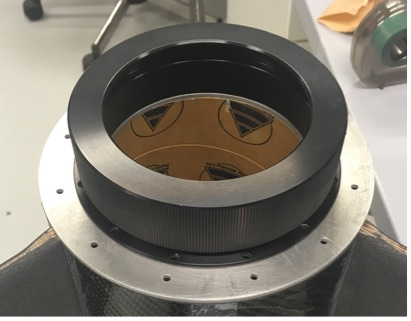
\includegraphics[width=0.3\textwidth]{img/motor_retainer.jpg}
        \caption{Motor Retainer and the Aluminum plate}
        \label{f:motor_retainer_2}
    \end{figure}


\paragraph{Payload}
\hfill \break
In the lower body of the rocket, there is 1U of payload 
consisting of 4kg of tungsten and a board with sensors used to track the lower body motion and shocks, referred to as the Logging Electronics. A Gopro and a PCB cameras are also placed to film the parachute deployment and the outside.
The Active Payload bay, placed in the Upper Body, consists of a 4U plywood box reinforced with glass fibre to withstand the loads. Inside the 4U wood box, a glider is mounted on a rail. Shortly after apogee, the glider will be ejected from the rocket using a spring. A more detailed description of the glider will be detailed in Section \ref{section:gliders}




\subsection{Recovery}
This subsystem implements a dual-event recovery concept of operations (CONOPS) with an initial deployment event at apogee and a main deployment event at 457m (1500ft) AGL. Figure \ref{f:recovery_conops} illustrates the recovery CONOPS.
\begin{figure}[h!]
 	\centering
        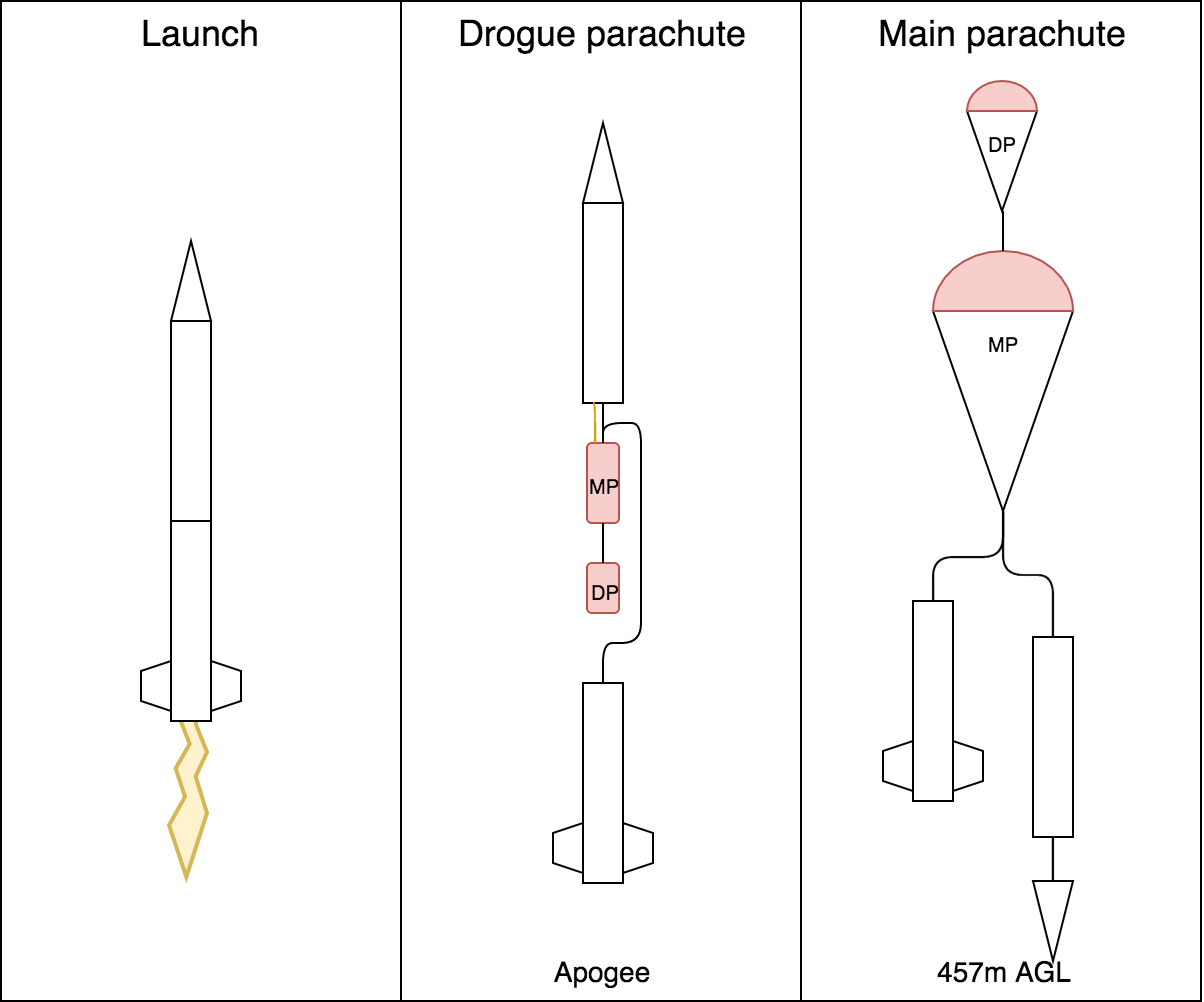
\includegraphics[width=0.45\textwidth]{img/recovery_conops_schema.png}
        \caption{Recovery CONOPS}
        \label{f:recovery_conops}
 \end{figure}

During the initial deployment, the rocket is separated and a drogue parachute is released to stabilize the attitude and reduce descent rate to 23-46 m/s (75-150ft/s).At 457m above ground level (AGL) the main deployment takes place where the main parachute is released from the parachute bag to reduce the rocket's descent rate to less than 9m/s (30ft/s) to prevent excessive damage upon impact. Recovery Avionics system triggers the deployment events when the preprogrammed deployment conditions are met by firing a pyrotechnical charge.

\paragraph{Initial Deployment System}
\hfill \break
The initial deployment is achieved by creating a pressure in the parachute bay and thus forcing the two rocket bodies to separate. The pressure is generated by puncturing a 23ml CO2 cartridge by a 0.2 ml black powder charge. The charge forces a puncture piston inside the cartridge seal to release the gas. This system is a COTS solution from Tinder Rocketry Recovery Solutions.
There are two redundant CO2 deployment systems each connected to two igniters. 2 redundant recovery electronic components are in charge of triggering the system and each of the two can trigger both systems. Recovery avionics is outlined later in this section.

\paragraph{Main Deployment System}
\hfill \break
The main parachute is stowed in the bag below the drogue parachute. The main parachute is held together by a wire which is cut at the programmed altitude. Then the load of the rocket pulls the main parachute out of the parachute bag. The setup is illustrated in Figure \ref{f:recovery_main_deployment}. The wire is cut by a shearing piston which is forced through the wire by a 0.1ml black powder charge.Two wire cutters are installed for redundancy, one per recovery electronics.

\begin{figure}[h!]
 	\centering
        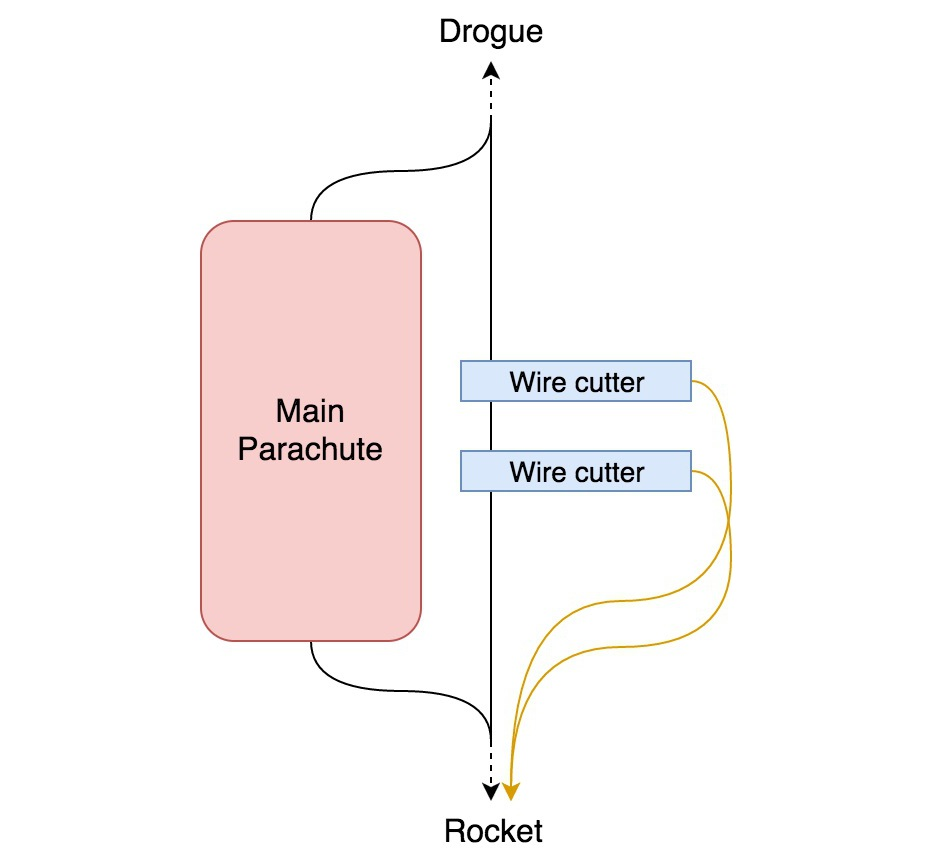
\includegraphics[width=0.45\textwidth]{img/recovery_main_deployment.jpg}
        \caption{Main Parachute Deployment}
        \label{f:recovery_main_deployment}
 \end{figure}

 \paragraph{Recovery Avionics}
 \hfill \break
The Recovery Avionics is designed for maximal reliability and features several levels of redundancy which is shown in Figure \ref{f:recovery_avionics_schema}. As required by the the competition rules, two redundant electronic systems are used, both of which are different COTS solutions.
The primary electronics is the AltimaxG3 from Rocketronics which features barometer and accelerometer sensors to estimate the altitude of the rocket. It uses a Kalman filter to estimate acceleration, speed and altitude of the rocket. This is a more robust solution especially when pressure fluctuations can be expected at a high velocity.
The backup electronics is the Raven3 from Featherweight Altimeters.
The primary electronics is programmed to detect the apogee and fire the two CO2 charges one after the other with a delay of 0.5 seconds. Then during descent it monitors air pressure until the main parachute deployment altitude is reached and initiates the deployment by using the wire cutter.
 The backup electronics is programmed as a timer to trigger the initial deployment after the predicted time to apogee from simulations. During descent it also detects the target altitude using a pressure sensor to trigger the main deployment

  \begin{figure}[h!]
 	\centering
        \includegraphics[width=0.5\textwidth]{img/recovery_avionics_schema.png}
        \caption{Recovery Avionics Schema}
        \label{f:recovery_avionics_schema}
 \end{figure}
  

\paragraph{Recovery Bay} 
 The recovery structure is made out of laser cut and milled plywood glued together with epoxy. It is screwed onto a circular bulkhead glued into the upper rocket tube. The connection to the parachute bay is made as airtight as possible by sealing holes with glue and using rubber washers.
Figure \ref{f:recovery_bay} shows the assembled recovery bay.
 \begin{figure}[h!]
 	\centering
        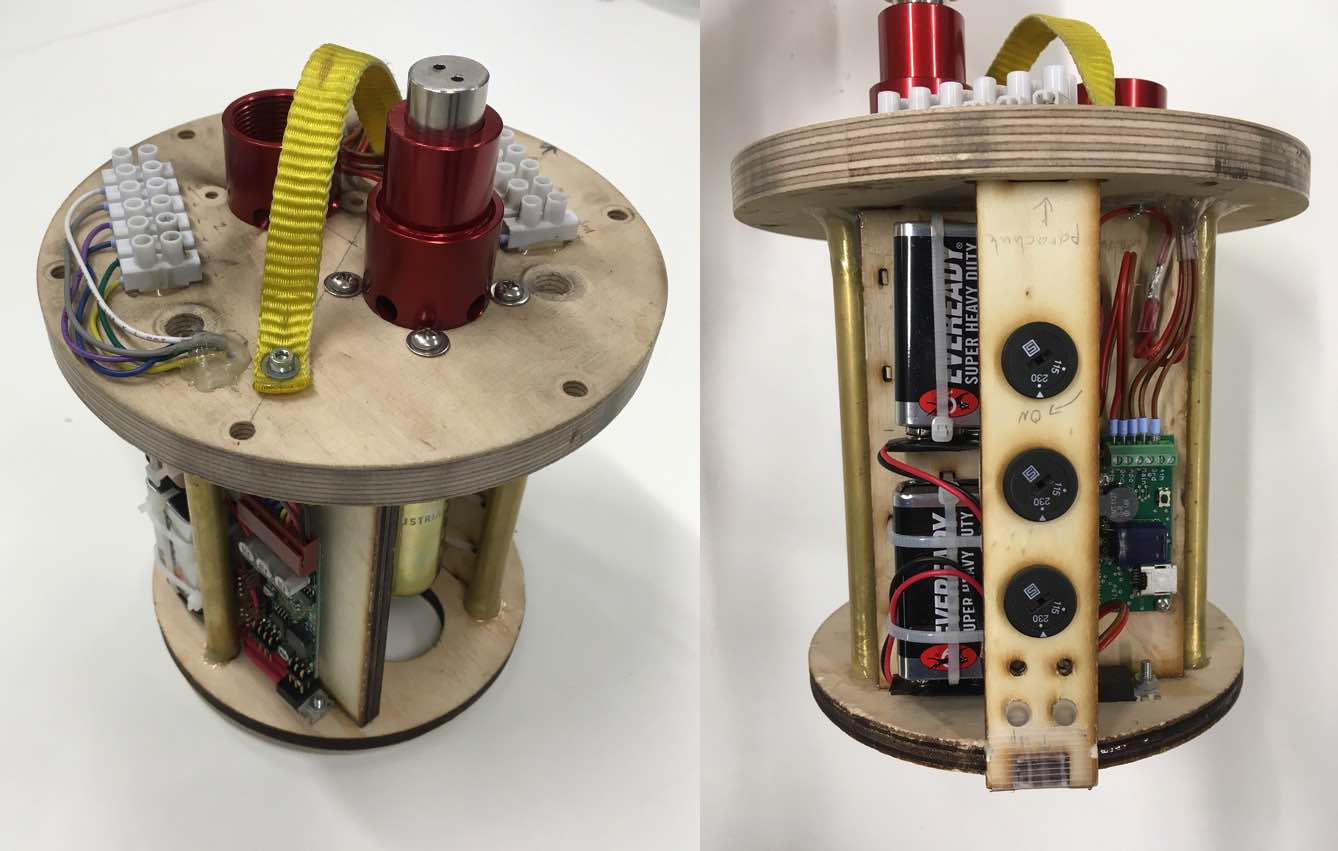
\includegraphics[width=0.45\textwidth]{img/recovery_bay.jpg}
        \caption{Recovery Bay}
        \label{f:recovery_bay}
 \end{figure}
 
 
\subsection{Avionics}
The avionics consist of 2 PCBs stacked together. The first one, referred to as the \textbf{Interface Board (IB)} shown in Figure \ref{f:avionics_ib}, is equipped with:
\begin{itemize}[noitemsep]
    \item an absolute pressure sensor for altitude measurement
    \item 2 differential pressure sensors for the Pitot tube
    \item an IMU
    \item a microcontroller (STM32F4 of STMicroelectronics)
    \item a GNSS receiver
    \item Xbee for telemetry downlink to the ground station
    \item 64 MB of flash memory for data logging
    \item interfaces such as 2 RS232 ports and USB port
\end{itemize}

The second PCB, the so called \textbf{Power Board (PB)}  shown in Figure \ref{f:avionics_pb}, is equipped with a voltage regulator that power all the nosecone avionics and up to 6 servo outputs.

All electronic components used for the avionics are automotive graded or better to ensure a proper working of the system under vibration and high temperature. Moreover, all the components were selected to be easily checked under microscope after soldering (e.g. no BGA chip are used as they usually require X-ray inspection).
The decision to split the avionics into 2 PCBs is made to overcome the limited space available and to avoid issues due to EMC. The buck converter on the PB can potentially generate a lot of EM perturbations, thus the sensitive parts such as the GNSS are placed away from it, namely on the IB.
As the rocket body is made of carbon fibre, the only RF transparent part of the rocket is the nosecone (made of fibre glass). Therefore, all the electronics components were integrated and placed there.

 \begin{figure}[h!]
 	\centering
        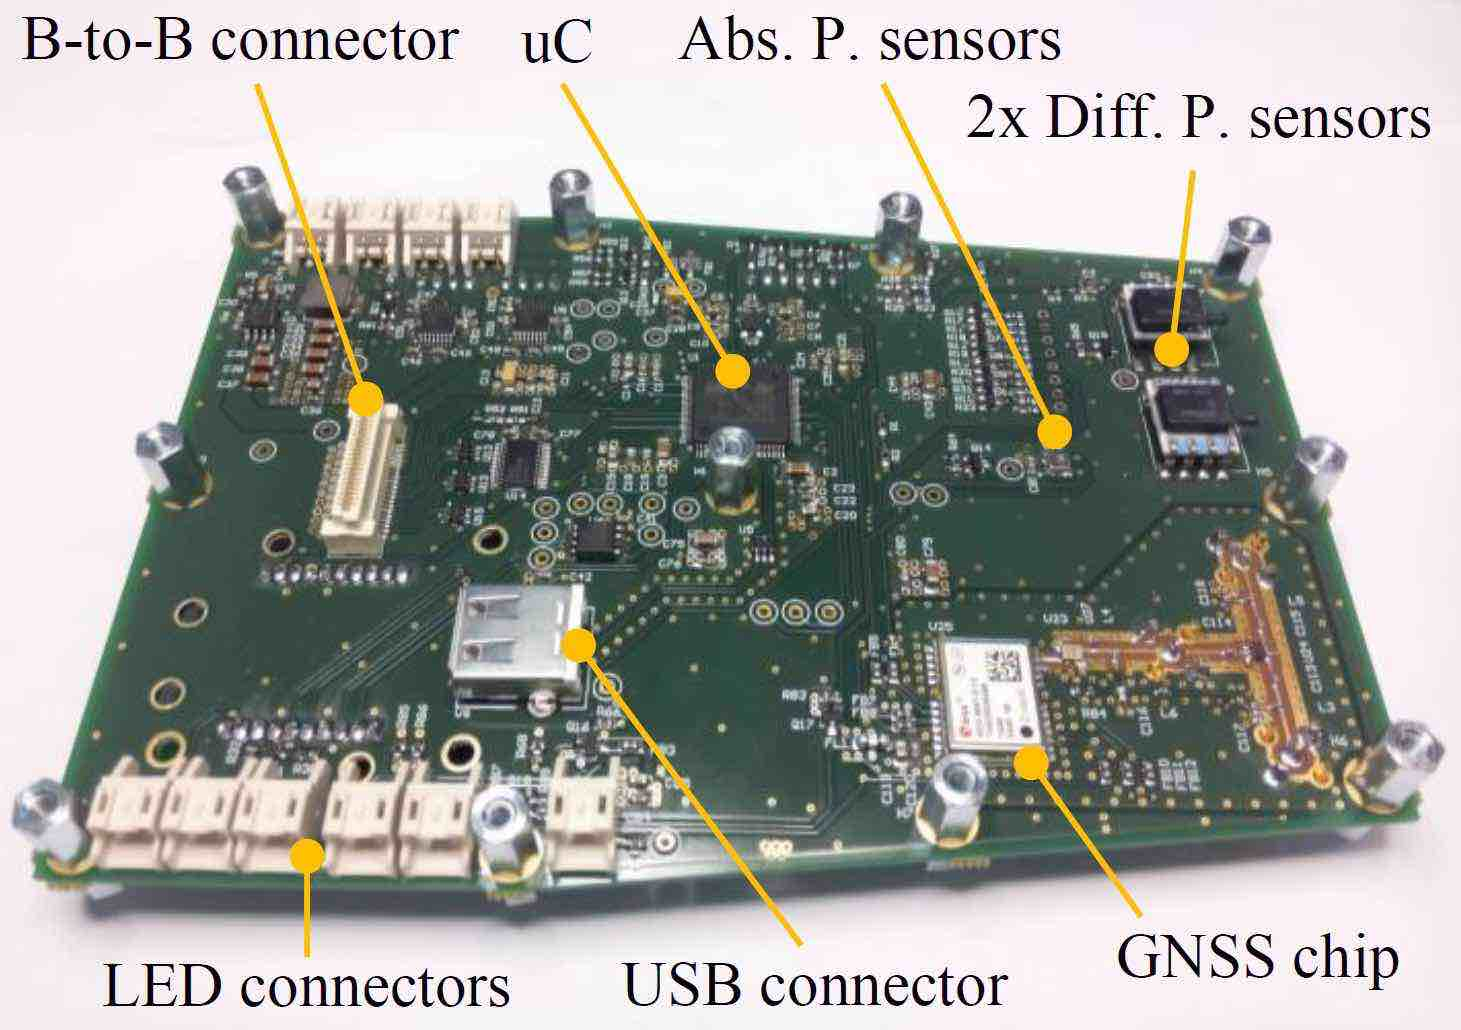
\includegraphics[width=0.45\textwidth]{img/AV_FIG_IB_top.jpg}
          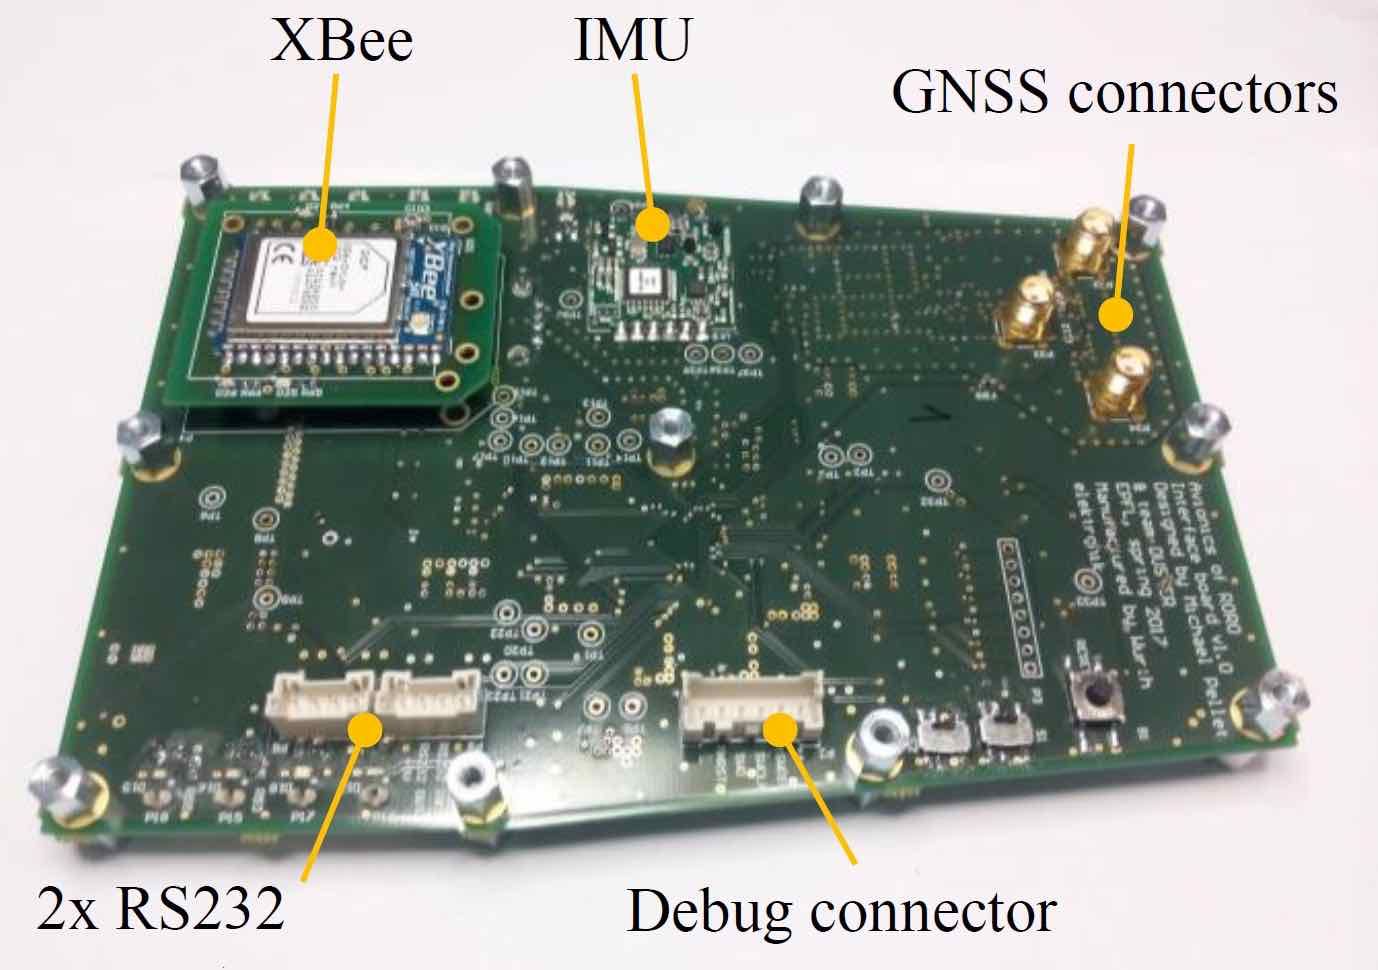
\includegraphics[width=0.45\textwidth]{img/AV_FIG_IB_bottom.jpg}
        \caption{Interface Board (IB) Top and Bottom)}
        \label{f:avionics_ib}
 \end{figure}
 
  \begin{figure}[h!]
 	\centering
        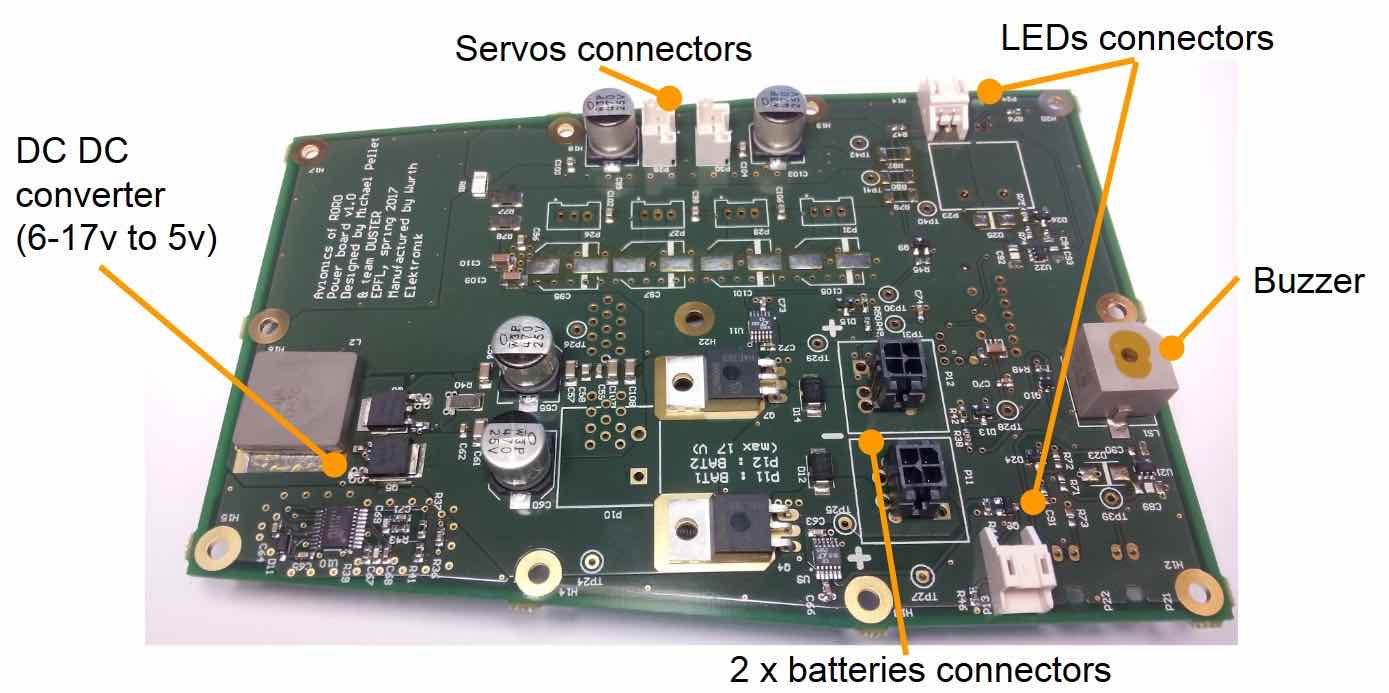
\includegraphics[width=0.45\textwidth]{img/AV_FIG_PB_top.jpg}
          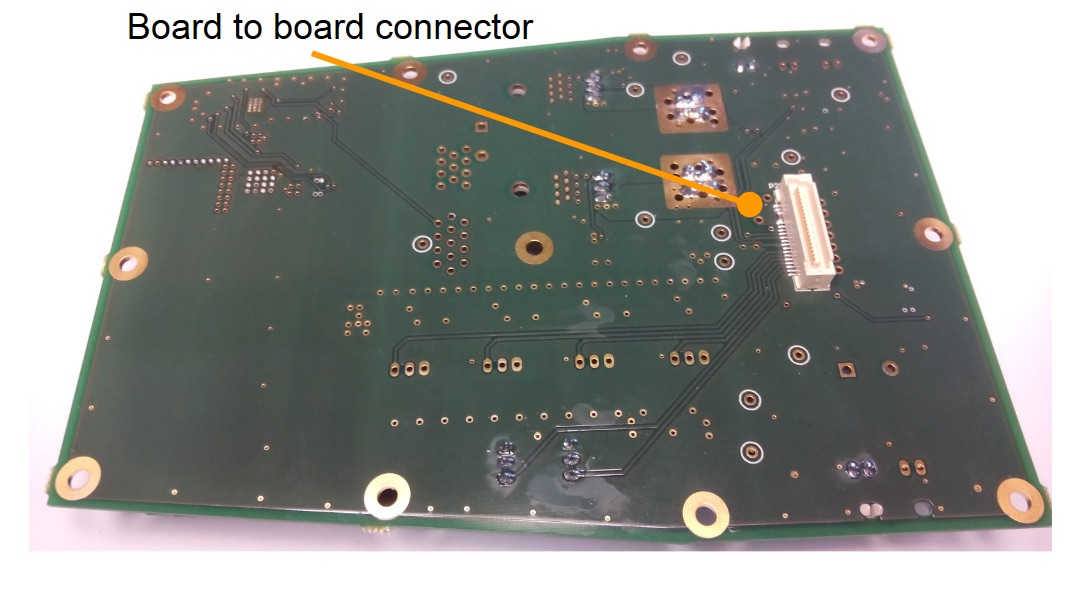
\includegraphics[width=0.45\textwidth]{img/AV_FIG_PB_bottom.jpg}
        \caption{Power Board (PB) Top and Bottom}
        \label{f:avionics_pb}
 \end{figure}

\paragraph{Sensors}
 \hfill \break
The Pitot tube uses 2 differential pressure sensors of Honeywell in parallel with different pressure range (0 to 6890Pa and 0 to 103350 Pa). This allows reduction of uncertainties at low speed (uncertainty of 6 m/s at 10 m/s) and ensures good performances at higher speed (uncertainty of 2m/s at 280m/s).
The IMU (3 Space High-G of Yost Labs) which is directly soldered on the IB can measure acceleration up to 24g and rate of turn up to 2000/s.
By using its integrated data possessing unit, it can directly output orientation (Euler angles, quaternions or rotation matrix) as well as acceleration, rate of turn, magnetic field and velocity increments with a data rate of up to 250 Hz.

The GNSS chip is a NEO-M8T of uBlox equipped with a SAW (surface acoustic waves) filter. As the telemetry antenna (XBee) is close to the 1st GNSS antenna, 2nd SAW filter (SF1186G of muRata) is placed just before the RF input in order to ensure an optimum operation of the GNSS (e.g. avoid jamming due to the XBee frequencies).There are 2 GNSS active antennas. One is placed at the back of the nose cone and is oriented toward the back of the rocket and the other one is placed at the front of the nose cone and is oriented toward the front of the rocket. The 2 GNSS active antennas are controlled via an RF switch on the IB. The first GNSS antenna is used during ascend of the rocket while the second one is used during the descent, after the deployment of the drogue parachute and the nosecone ejection.

\paragraph{Telemetry Downlink}
 \hfill \break
For the telemetry downlink, a 900MHz XBee (XB9X-DMUS-001 of Digi International) is placed on the IB and connected to a 2.1dBi omni antenna. Second XBee is directly connected to the ground station which uses a high gain Yagi antenna (23dB) that is manually oriented towards the rocked during flight. This configuration ensures a good power margin (45dBm) above the sensitivity level of the receiver when at maximum theoretical distance (5 km). The XBee on the IB is fixed with 2 screws and is easily accessible and replaceable in order to replace it according to the country of operation (868 MHz for CH and 900 MHz for the US). Using XBee at 2.4GHz (which is legal for both CH and US) was not an option as they don't have a sufficient communication range

\paragraph{Actuators}
 \hfill \break
The PB is equipped with 6 servo outputs, each allowing to control a high power servo. These outputs could be used in the future to implement an active control system of the rocket. In RORO I, 2 of these outputs are used. One is used to control the mechanism which ejects the nosecone while the other is used to control the release of the payload (the glider). 

\paragraph{Power Supply}
 \hfill \break
A high power buck converter from Texas Instrument is implemented on the PB. This device allows to power the avionics with 5 VDC with up to 15 A with 2S to 4S (6V to 17V) LiPo batteries. The PB is also equipped with 2 ideal diodes IC that allow to use 2 batteries in parallel for redundancy. In the case of RORO I, 2 3S, 1800 mAh LiPo are used. 

\paragraph{Software}
 \hfill \break
The software implemented in the avionics for RORO I mainly integrates the following functionalities: Data logging in the flash memory of the measurements performed by the sensors, detection of the launch of the rocket (with a threshold on the acceleration data from the IMU), sending the data of the GNSS (position) to the ground station via the XBee module, detection of the apogee of the rocket in order to open the nosecone 5 seconds after this event using a servo and switching to the 2nd GNSS antenna after the deployment of the nosecone. Five seconds after the deployment of the nosecone, second servo is trigged which allows the deployment of the payload.

\subsubsection{Mechanical Design and Manufacturing}
\paragraph{Mechanical Integration of the Avionics in the Nosecone}
 \hfill \break
The mechanical structure is designed with the idea of having the avionics easily accessible on the field. The 2 avionics PCBs are staked between 2 CNC machined plates of 3 mm tick plywood and fixed together with PCB spacers. On each plywood plate, gliding structures made out on plywood are glued. This assembly, called the avionic drawer (AD), can be easily slided into the avionic rack (AR) which is a structure made of several parts of CNC machined 6 mm tick plywood fixed to the control panel. To secure the AD, the aluminum GNSS ground plane of the 1st GNSS antenna is fixed on the top of it with nuts to two M5 threaded rods. These 2 threaded rods pass trough the avionic rack and are fixed to the control panel. On the control panel side, a hook is fixed at the end of each threated rod. These hooks are used to fix the rope that link the nosecone to the upper body bulkhead. The structure made of the control panel on which the AR together with the AD is fixed can be slided into the nosecone and be fixed with 6 M3 screws to a plywood crown glued with epoxy to the nosecone. The Avionics Bay inside the nosecone is depicted in Figure \ref{f:avionics_bay}.

  \begin{figure}[h!]
 	\centering
        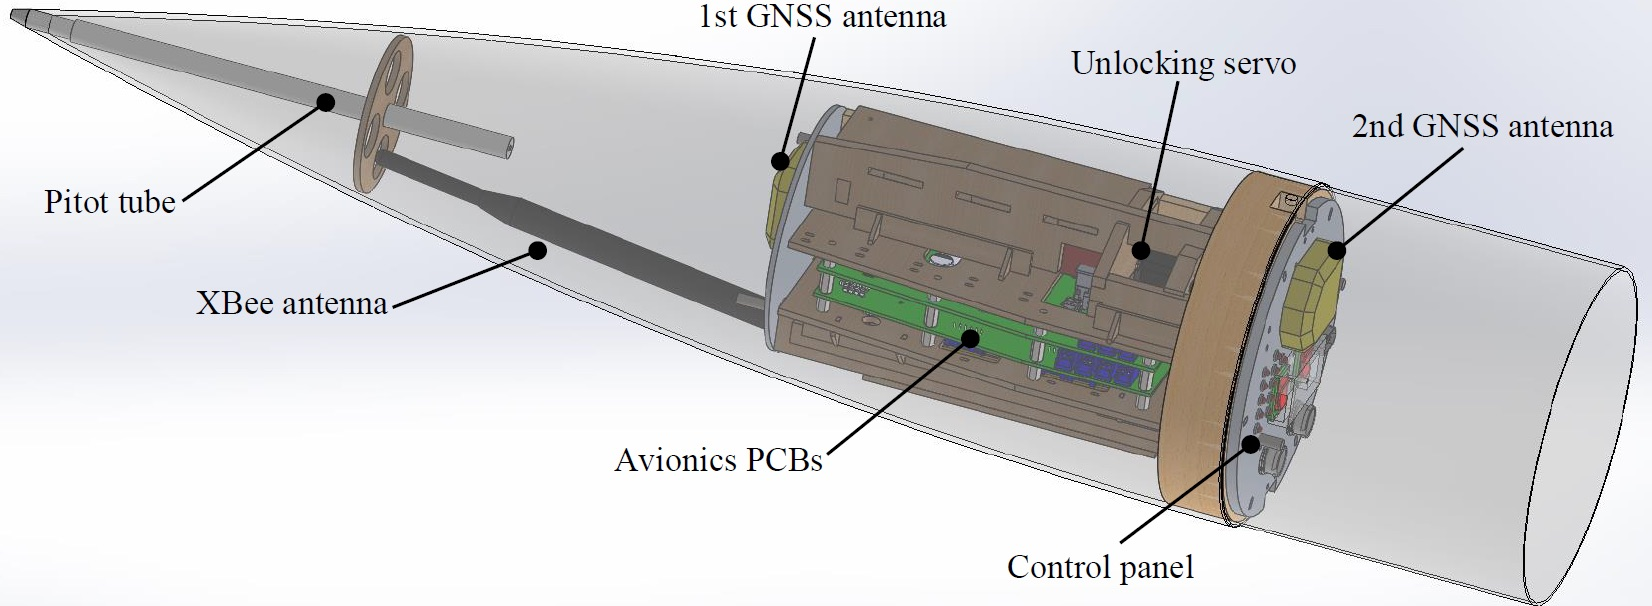
\includegraphics[width=0.45\textwidth]{img/AV_FIG_CAD_nosecone.jpg}
        \caption{Avionics Bay inside the Nosecone}
        \label{f:avionics_bay}
 \end{figure}

\paragraph{Nosecone Deployment System}
 \hfill \break
\textit{Note: in the following paragraph, everything noted in parenthesis refers to the Figure \ref{f:av_deployment_sys}}

In order to get the satellite fix for the GNSS after apogee, the nosecone needs to be deployed. Moreover, this makes an opening in the upper body that allows to deploy the payload. So, to ensure the deployment of the nosecone, an ejection system was designed and manufactured that take into account the fact that the
main part of the volume below the nosecone is occupied by the payload.

The designed and manufactured system consist of 2 aluminum U-profiles (6.) fixed to the bulkhead (2.) of the upper body (1.). At the upper end of the u-profiles, a hook is fixed (7.) that is used by the looking system to secure the nosecone (5.). A gliding structure (3.) made out of 2 bigger aluminum U-profiles joined together with 4 arcs cut out of a phenolic tube can slide into the upper body.
In the smaller U-profiles (6.), a traction spring (4.) is fixed just bellow the hook (7.), the other end of the spring is fixed on the gliding structure (3.). So, when the nosecone is put in place, the upper part of the gliding structure comes in contact with the lower end of the nosecone and, thus, the gliding structure is pushed in the upper body which loads the 2 springs. When fully loaded, the 2 spring produce a total force of c.a. 100N. When the nosecone is released (thanks to the locking system) the gliding structure pushes it away from the upper body.

  \begin{figure}[h!]
 	\centering
        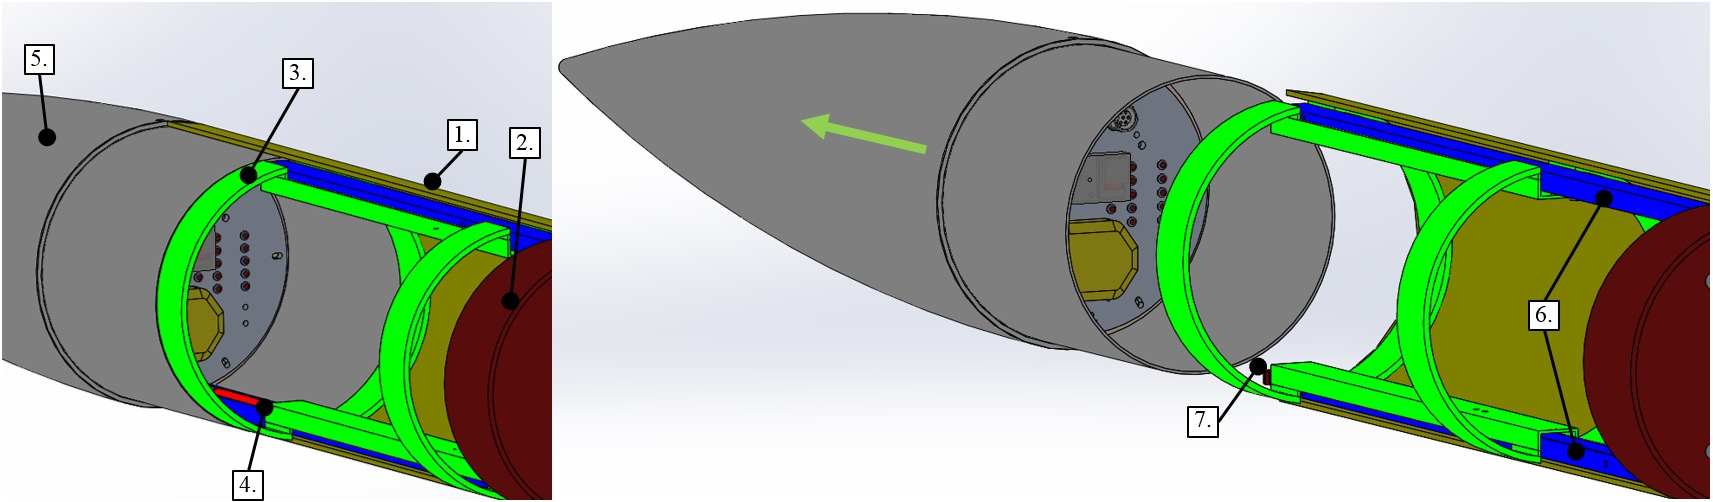
\includegraphics[width=0.45\textwidth]{img/AV_FIG_CAD_depl_sys_1.jpg}
        \caption{Deployment System of the Nosecone. LEFT: In place on the upper body. RIGHT: after deployment. (for clarity, payload is not shown)}
        \label{f:av_deployment_sys}
 \end{figure}

\paragraph{Nosecone Locking System}
 \hfill \break
\textit{Note: in the following paragraph, everything noted in parenthesis refers to the Figure \ref{f:av_locking_sys}}.

To secure the nosecone in place during the ascend of the rocket, a locking system was designed and manufactured. This system consist out of 2 steel pins of 6 mm diameter (2. and 3.) loaded with a compressive spring (4.) that can slide in a structure (1.) fixed to the control panel of the nosecone. An ?inverted? came wheel (5.) controlled with a servo that is fixed to the AR is used to move the 2 pins forth and back. When locked, the end of the 2 pins goes in a hook (7.) fixed to each outer rail (6.) of the
deployment system. When unlocked, the steel rods are retracted and comes out of the hooks. 
This configuration, with an inverted came wheel, allows to unlock the nosecone from the outside even if there is a failure of the servo or the avionics. Indeed, the axis of the 2 locking steel rods is aligned with the 2 holes (8.) made in the nosecone for Pitot tube?s static pressure measurement, thus, the locking system can be unlocked using 2 screwdriver to push the pins inside the nosecone

  \begin{figure}[h!]
 	\centering
        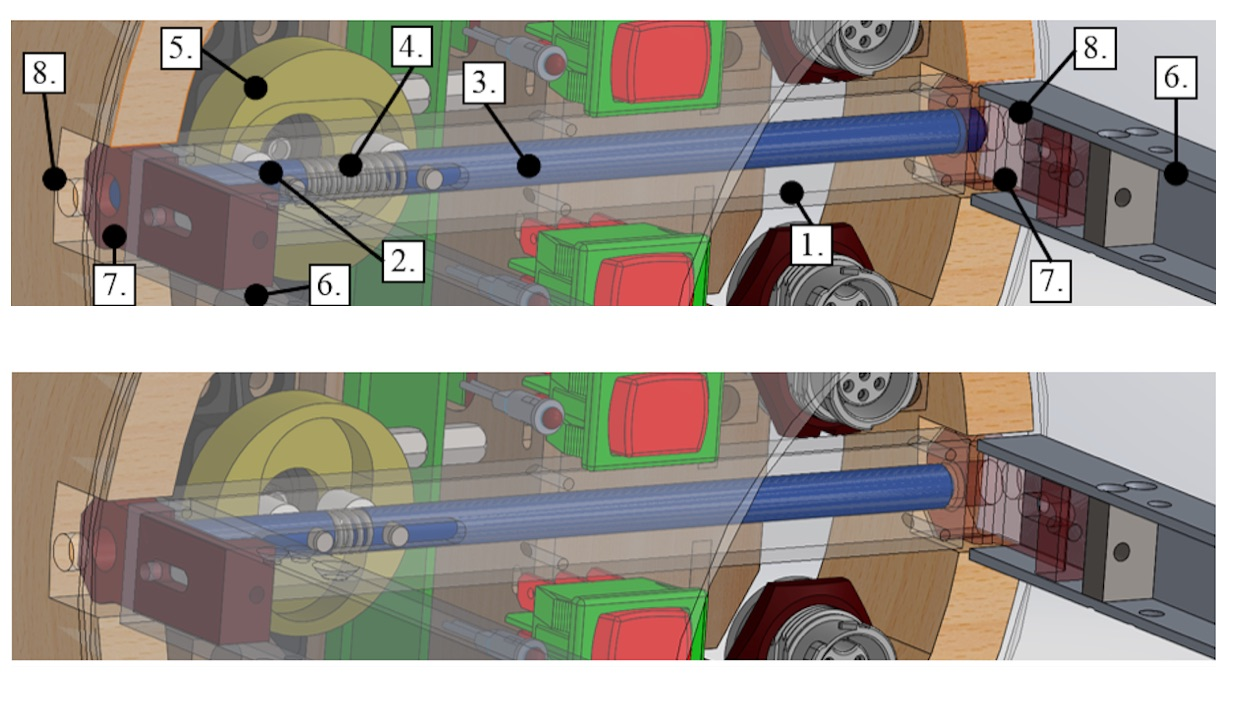
\includegraphics[width=0.45\textwidth]{img/AV_FIG_CAD_lockingsystem_22.jpg}
        \caption{Locking System of the Nosecone. Top: locked, Bottom: unlocked}
        \label{f:av_locking_sys}
 \end{figure}




\section{Gliders}

\subsection{General Overview}

Each team can choose an arbitrary payload to design and build. The team decided to develop long-term a set of gliders that are, once deployed from the rocket, flying back to the ground in formation. 


For this year, the team prepared a technology demonstrator consisting of only one glider deployed at apogee. This can be extrapolated for a fleet of 7 gliders. The challenge of building more gliders lies in fitting them into a constrained space in the rocket. 

\paragraph{Motivation for choosing the payload}
\hfill \break
Rovers such as Curiosity or Spirit have studied Martian terrain and sent back scientific data which may answer questions regarding the origin of life. However, in-situ atmospheric measurements of Mars on longer distances are missing. In order to solve this need, gliders, balloons, or powered planes should overfly Mars and land in areas where rovers cannot. Several projects are proposed by NASA in these directions such as the Preliminary Research Aerodynamic Design to Land on Mars (Prandtl-m) Airplane which aims to be released from a 3U CubeSat and do a 1-hour descent onto the surface of Mars.

Inspired by the Prandtl-m project, our team aimed to design and build an autonomous glider for the Spaceport America Cup competition, and learn more about the flight dynamics and control of such a complex system.

% ref
% @misc{mars,
%   title = {Could This Become the First Mars Airplane?},
%   howpublished = {\url{https://www.nasa.gov/centers/armstrong/features/mars_airplane.html}},
%   note = {Accessed: 2016-07-06}
% }

\begin{table}[h!]
\centering
\begin{tabular}{|p{0.9\columnwidth}|}
\hline
    The payload shall weight 8.8 lb (3.9 kg). \\ \hline
    The payload shall consist of a glider and ballast.  \\ \hline
    The glider shall be deployed at apogee. \\ \hline
    The glider shall deploy its wings passively once ejected from the rocket. \\ \hline
    The glider shall be equipped with an RTK (Real Time Kinematic) GPS used for navigation. \\ \hline
    The glider shall be equipped with a Commercial-Off-The-Shelve autopilot and a pitot tube \\ \hline
    The glider's battery life shall be 1.5 hours. \\ \hline
\end{tabular}
\caption{Top Level Requirements for the payload}
\label{table:se_topLevelR}
\end{table}


\subsection{Design and Manufacturing of ONE glider-SORINA}
%Pictures from report here

Due to space constraints, the glider was chosen to be a flying wing with the wings folded in front. XFLR simulations experiments with different airfoils, wing span, wing sweep were performed until the acceptable flight parameters were obtained. The final airfoil is a MH45, with improved (3\%) reflex.

The plane parameters are presented in Table X.


The optimal flight data is presented in Table Y.


\subsection{Design and Manufacturing of a fleet of gliders-SORINA}
%Concept TBD in solidworks 

\subsection{Navigation and Control of the fleet of gliders}
\label{subsection:navcontrol}
%Ultrawide beacons 
%Formation
%Check for alternative options, instead of GPS



\section{Conclusions}
\section{Outlook}
%Maybe talk about airbrakes, active control, etc.

\end{document}